% -*- mode: latex; mode: visual-line; fill-column: 9999; coding: utf-8 -*-

\section{Reproducibility and Performance Comparison on Different Clusters}
\label{sec:clusters}

In this section we compare the performance of the RMSD task on different HPC resources (Table \ref{tab:sys-config}) to examine the robustness of the methods we used for our performance study and to ensure that the results are general and independent from the specific HPC system.
Scripts and instructions to set up the computational environments and reproduce our computational experiments are provided in a git repository as described in section \ref{sec:methods}.

In \ref{sec:supplement}, we demonstrated that stragglers occur on \emph{PSC Bridges} (Figure \ref{fig:MPIwithIO-Bridges}) and \emph{LSU SuperMIC} (Figure \ref{fig:MPIwithIO-SuperMIC}) in a manner similar to the one observed on \emph{SDSC Comet} (section \ref{sec:RMSD}).
We performed additional comparisons for several cases discussed previously, namely (1) splitting the trajectories with blocking collective communications in MPI, (2) splitting the trajectories with Global Arrays for communications, and (3) MPI-based parallel HDF5.

\subsection{Splitting the Trajectories}
Figure \ref{fig:MPI-splitting-clusters} shows the strong scaling of the RMSD task on different HPC resources.  
Splitting the trajectories with Global Arrays for communication resulted in very good scaling performance on \emph{LSU SuperMIC}, similar to the results obtained on \emph{SDSC Comet}.
The results with MPI blocking collective communication (instead of Global Arrays) were also comparable between the two clusters, with scaling far from ideal due to the communication cost (see section \ref{splitting-traj} and Figures \ref{fig:MPIranks-split} and \ref{fig:MPIwithIO-split-SuperMIC}). 
Overall, the scaling of the RMSD task is better on \emph{LSU SuperMIC} than on \emph{SDSC Comet} and the performance gap increased with increasing core number.
The results on \emph{LSU SuperMIC} confirmed the conclusion obtained on \emph{SDSC Comet} that at least in this case Global Arrays performed better than MPI blocking collective communication.

\begin{figure}[!htb]
  \centering
  \begin{subfigure}{.49\textwidth}
    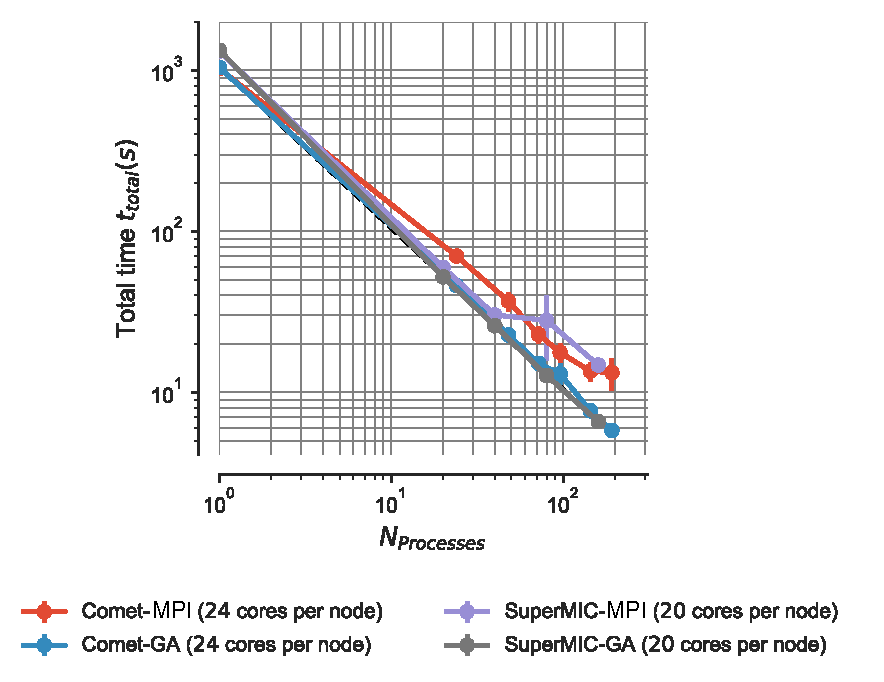
\includegraphics[width=\linewidth]{figures/Comparison_t-tot-clusters_Splitting_edited.pdf}
    \caption{Scaling total}
    \label{fig:MPIscaling-clusters-splitting}
  \end{subfigure}
  \hfill
  \begin{subfigure}{.49\textwidth}
    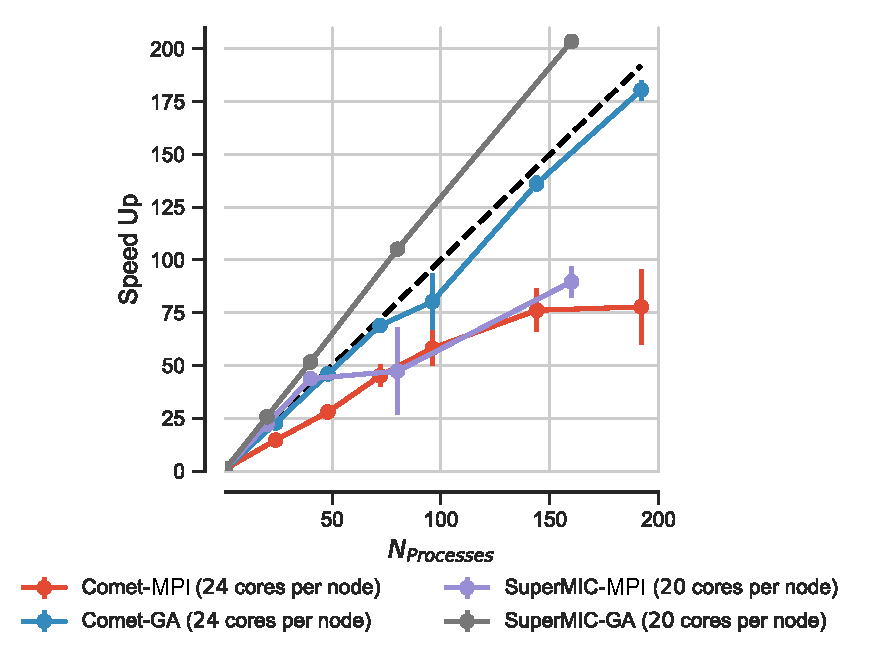
\includegraphics[width=\linewidth]{figures/Comparison_speed-up-clusters_Splitting_edited.pdf}
    \caption{Speed-up}
    \label{fig:MPIspeedup-clusters-splitting}
  \end{subfigure}
  \bigskip

  \begin{subfigure}{0.7\textwidth}
    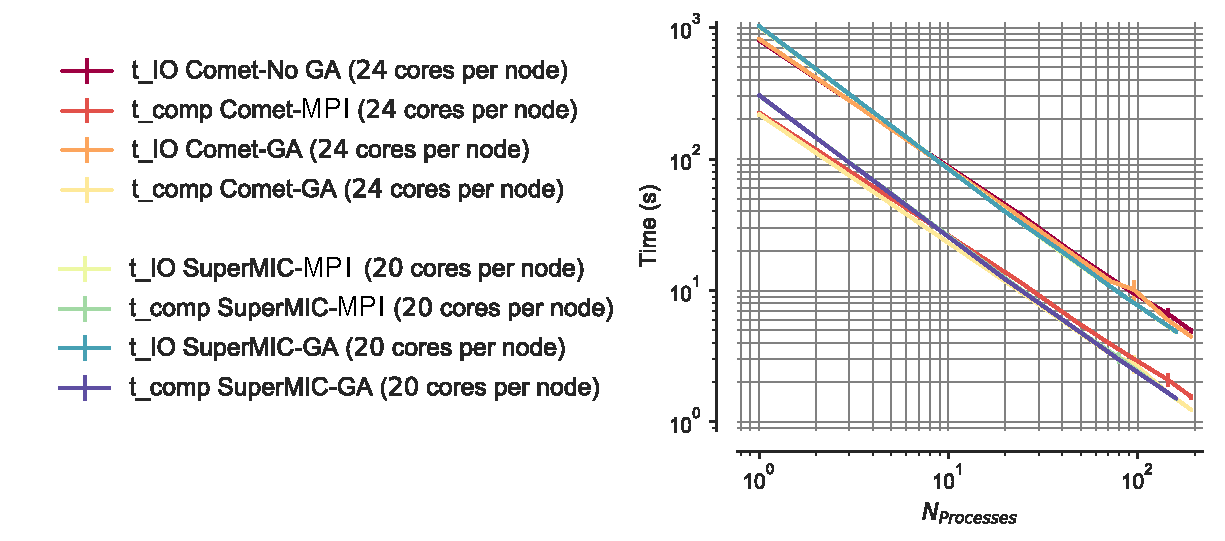
\includegraphics[width=\linewidth]{figures/Clusters_IO_compute_scaling_splitting_edited.pdf}
    \captionsetup{format=hang}
    \caption{Scaling of \tcomp and \tIO.}
    \label{fig:compute-IO-scaling-clusters-splitting}
  \end{subfigure}
  \caption{Comparison of the performance of the RMSD task across different clusters (\emph{SDSC Comet}, \emph{LSU SuperMIC}) when the trajectories are split (\emph{subfiling}).
    Results were communicated back to rank 0 either with MPI collective communications (label ``MPI'') or using \package{Global Arrays} (label ``GA'').
    Five repeats were performed to collect statistics.
    The error bars show the standard deviation with respect to the mean.}
\label{fig:MPI-splitting-clusters}
\end{figure} 

\subsection{MPI-based Parallel HDF5}

Figure \ref{fig:MPIwithIO-clusters} shows the scaling on \emph{SDSC Comet}, \emph{LSU SuperMIC}, and \emph{PSC Bridges} using MPI-based parallel HDF5.  
Performance on \emph{SDSC Comet} and \emph{LSU SuperMIC} was very good with near ideal linear strong scaling.
The performance on \emph{PSC Bridges} was sensitive to how many cores per node were used.
Using all 28 cores in a node resulted in poor performance but decreasing the number of cores per node and equally distributing processes over nodes improved the scaling (Figure \ref{fig:MPIwithIO-clusters}), mainly by reducing variation in the I/O times.

The main difference between the runs on \emph{PSC Bridges} and \emph{SDSC Comet}/\emph{LSU SuperMIC} appeared to be the variance in \tIO (Figure \ref{fig:compute-IO-scaling-clusters}).
The I/O time distribution was fairly small and uniform across all ranks on \emph{SDSC Comet} and \emph{LSU SuperMIC} (Figures \ref{fig:hdf5-SuperMIC} and \ref{fig:MPIranks-hdf5}).
However, on \emph{PSC Bridges} the I/O time was on average about two and a half times larger and the I/O time distribution was also more variable across different ranks (Figure \ref{fig:hdf5-bridge}).  

\begin{figure}[!htb]
  \centering
  \begin{subfigure}{.49\textwidth}
    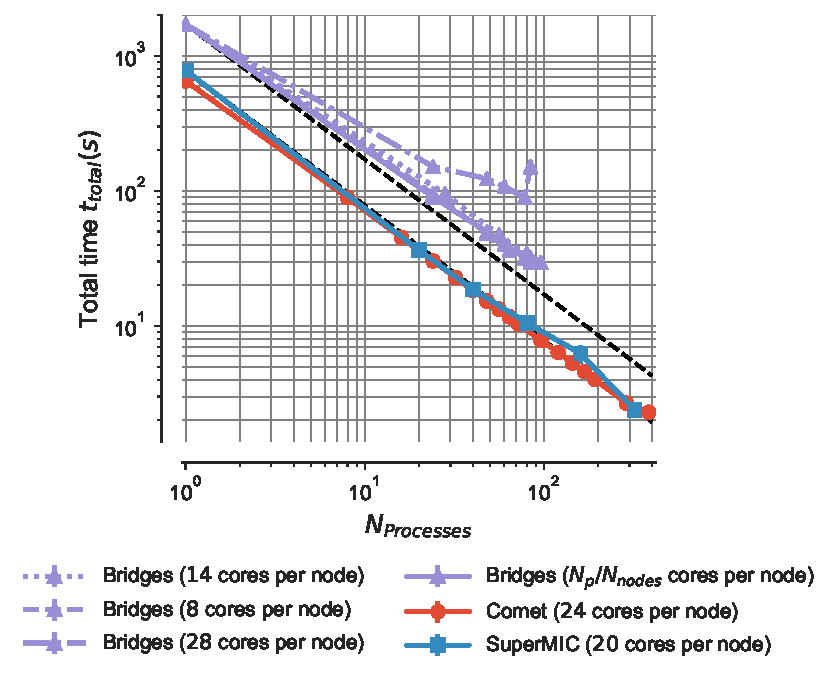
\includegraphics[width=\linewidth]{figures/Comparison_t-tot-clusters.pdf}
    \caption{Scaling total}
    \label{fig:MPIscaling-clusters}
  \end{subfigure}
  \hfill
  \begin{subfigure}{.49\textwidth}
    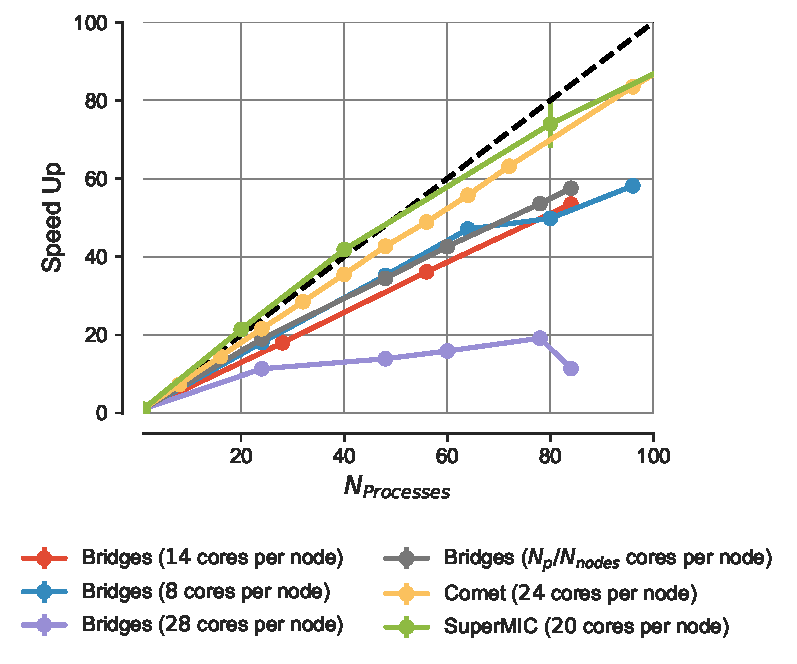
\includegraphics[width=\linewidth]{figures/Comparison_speed-up-clusters.pdf}
    \caption{Speed-up}
    \label{fig:MPIspeedup-clusters}
  \end{subfigure}
  \bigskip
  
  \begin{subfigure} {\textwidth}
    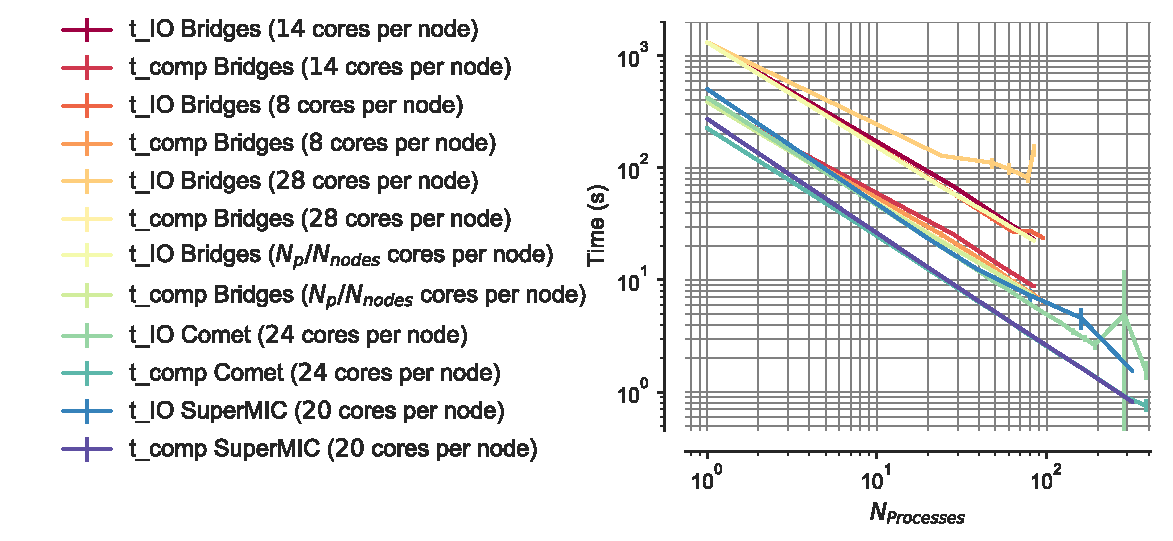
\includegraphics[width=\linewidth]{figures/Clusters_IO_compute_scaling_edited.pdf}
    \captionsetup{format=hang}
    \caption{Scaling of \tcomp and \tIO}
    \label{fig:compute-IO-scaling-clusters}
  \end{subfigure}
  \caption{Comparison of the performance of the RMSD task across different clusters (\emph{SDSC Comet}, \emph{PSC Bridges}, \emph{LSU SuperMIC}) with MPI-IO.
    Data were read from a shared HDF5 file instead of an XTC file, using MPI independent I/O in the PHDF5 library.
    Results were communicated back to rank 0.
    $N_{\text{P}}/N_{\text{nodes}}$ indicates that number of processes used for the task were equally distributed over all compute nodes.
    Five repeats were performed to collect statistics.
    The error bars show standard deviation with respect to mean.
    In (b) only results up to 100 cores are shown to simplify the comparison; see Fig.~\protect\ref{fig:MPIspeedup-hdf5} for \emph{SDSC Comet} and Fig.~\protect\ref{fig:comparison_efficiency_SuperMIC} for \emph{LSU SuperMic} data.
  }
\label{fig:MPIwithIO-clusters}
\end{figure} 

\begin{figure}[!htb]
  \centering
  \begin{subfigure}{.49\textwidth}
    \includegraphics[width=\linewidth]{figures/Bridge-MPI-IO-BarPlot-rank-comparison_78_5.pdf}
    \caption{\emph{PSC Bridges}}
    \label{fig:hdf5-bridge}
  \end{subfigure}
  \bigskip
  \begin{subfigure} {.49\textwidth}
    \includegraphics[width=\linewidth]{figures/SuperMIC-MPI-IO-BarPlot-rank-comparison_80_5.pdf}
    \caption{\emph{LSU SuperMIC}}
    \label{fig:hdf5-SuperMIC}
  \end{subfigure}
  \caption{Examples of timing per MPI rank for the RMSD task with MPI-based parallel HDF5 on (a) \emph{PSC Bridges} and (b) \emph{LSU SuperMIC}.
    Five repeats were performed to collect statistics and these were typical data from one run of the five repeats. Compute \tcomp, read I/O \tIO, communication \tcomm, ending the for loop $t_{\text{end\_loop}}$,  opening the trajectory $t_{\text{opening\_trajectory}}$, and overheads $t_{\text{overhead1}}$, $t_{\text{overhead2}}$ per MPI rank; see Table \ref{tab:notation} for definitions.}
  \label{fig:MPIwithIO-clusters-rank}
\end{figure} 

\subsection{Comparison of Compute and I/O Scaling Across Different Clusters}
A full comparison of compute and I/O scaling across different clusters for different test cases and algorithms is shown in Table \ref{tab:comp-IO-scaling}. 
For MPI-based parallel HDF5, both the compute and I/O time on \emph{Bridges} were consistently larger than their corresponding values on \emph{SDSC Comet} and \emph{LSU SuperMIC}.
For example, with one core the corresponding compute and I/O time were $\tcomp = 387~\text{s}$, $\tIO = 1318~\text{s}$ versus $225~\text{s}$, $423~\text{s}$ on \emph{SDSC Comet} and $273~\text{s}$, $503~\text{s}$ on \emph{LSU SuperMIC}.
This performance difference became larger with increasing core number.
When the trajectories were split and Global Arrays was used for communication both \emph{SDSC Comet} and \emph{LSU SuperMIC} showed similar performance.

Overall, the results from \emph{SDSC Comet} and \emph{LSU SuperMIC} are consistent with each other.
Performance on \emph{PSC Bridges} seemed sensitive to the exact allocation of cores on each node but nevertheless the approaches that decreased the occurrence of stragglers on \emph{SDSC Comet} and \emph{LSU SuperMIC} also improved performance on \emph{PSC Bridges}.
Thus, the findings described in the previous sections are valid for a range of different HPC clusters with Lustre file systems.

\begin{sidewaystable}[hp]
\centering
\caption
{Comparison of the compute and I/O scaling for different test cases and number of processes.
  Five repeats were performed to collect statistics.
  The mean value and the standard deviation with respect to mean are reported for each case.}
\label{tab:comp-IO-scaling}  
\begin{adjustbox}{max width=\textwidth}
\begin{tabular}{c c c c c c c c c c c c}
  \toprule
 \multicolumn{10}{r}{\bfseries $N_{Processes}$} \\
\cmidrule(r){5-12}
           \bfseries\thead{Cluster} & \bfseries\thead{Gather} & \bfseries\thead{File Access} & \bfseries\thead{Time} & \bfseries\thead{Serial} & \begin{tabular}{c} \bfseries\thead{Comet:} 24 \\ \bfseries\thead{Bridges:} 24 \\ \bfseries\thead{SuperMIC:} 20 \end{tabular}  & \begin{tabular}{c} \bfseries\thead{Comet:} 48 \\ \bfseries\thead{Bridges:} 48 \\ \bfseries\thead{SuperMIC:} 40 \end{tabular} & \begin{tabular}{c} \bfseries\thead{Comet:} 72 \\ \bfseries\thead{Bridges:} 60 \\ \bfseries\thead{SuperMIC:} 80 \end{tabular} & \begin{tabular}{c} \bfseries\thead{Comet:} 96 \\ \bfseries\thead{Bridges:} 78 \end{tabular} & \begin{tabular}{c} \bfseries\thead{Comet:} 144 \\ \bfseries\thead{Bridges:} 84 \\ \bfseries\thead{SuperMIC:} 160\end{tabular} & \bfseries\thead{Comet: 192} & \begin{tabular}{c} \bfseries\thead{Comet:} 384 \\  \bfseries\thead{SuperMIC:} 320\end{tabular}\\
  \midrule
    Comet & MPI & Single & \begin{tabular}{c} \tIO \\ \tcomp  \end{tabular} & \begin{tabular}{c} $791 \pm 5.22$ \\ $225 \pm 5.4$ \end{tabular} & \begin{tabular}{c} $49 \pm 3.45$ \\ $11 \pm 0.75$ \end{tabular} & \begin{tabular}{c} $29 \pm 1.3$ \\ $6 \pm 0.35$ \end{tabular} & \begin{tabular}{c} $26 \pm 9.19$ \\ $4 \pm 0.48$ \end{tabular} & -- & -- & -- & --\\  
  \midrule
    Bridges & MPI & Single & \begin{tabular}{c} \tIO \\ \tcomp  \end{tabular} & \begin{tabular}{c} $770 \pm 10.8$ \\ $221 \pm 3.9$ \end{tabular} &  \begin{tabular}{c} $38 \pm 0.84$ \\ $11 \pm 0.43$ \end{tabular} & \begin{tabular}{c} $33 \pm 19.4$ \\ $6 \pm 0.32$ \end{tabular} & \begin{tabular}{c} $15 \pm 1.6$ \\ $4 \pm 0.18$ \end{tabular} & -- & -- & -- & --\\  
  \midrule
    SuperMIC & MPI & Single & \begin{tabular}{c} \tIO \\ \tcomp  \end{tabular} & \begin{tabular}{c} $1014.51 \pm 2.94$ \\ $303.85 \pm2.3$ \end{tabular} & \begin{tabular}{c} $48.08 \pm 0.35$ \\ $14.56 \pm 0.14$ \end{tabular} & \begin{tabular}{c} $24.5 \pm 0.79$ \\ $7.4 \pm 0.25$ \end{tabular} & \begin{tabular}{c} $12 \pm 0.31$ \\ $3.7 \pm 0.12$ \end{tabular} & -- & \begin{tabular}{c} $6.24 \pm 0.38$ \\ $1.8 \pm 0.04$ \end{tabular} & -- & --\\  
  \midrule
    Comet & GA & Single & \begin{tabular}{c} \tIO \\ \tcomp \end{tabular} & \begin{tabular}{c} $820 \pm 18.49$ \\ $219 \pm 9.8$ \end{tabular} & \begin{tabular}{c} $41 \pm 8.99$ \\ $10 \pm 0.3$ \end{tabular} & \begin{tabular}{c} $23 \pm 4.14$ \\ $5 \pm 0.48$ \end{tabular} & \begin{tabular}{c} $15 \pm 2.06$ \\ $3 \pm 0.54$ \end{tabular} & -- & -- & -- & --\\
  \midrule
    Comet & MPI & Splitting & \begin{tabular}{c} \tIO \\ \tcomp \end{tabular} & \begin{tabular}{c} $799 \pm 5.22$ \\ $225 \pm 5.4$ \end{tabular} & \begin{tabular}{c} $37 \pm 1.22$ \\ $11 \pm 0.31$ \end{tabular} & \begin{tabular}{c} $18 \pm 0.18$ \\ $5 \pm 0.07$ \end{tabular} & \begin{tabular}{c} $12 \pm 0.14$ \\ $3 \pm 0.04$ \end{tabular} & \begin{tabular}{c} $9 \pm 0.3$ \\ $3 \pm 0.11$ \end{tabular} & \begin{tabular}{c} $6  \pm 0.66$ \\ $2 \pm 0.23$ \end{tabular} & \begin{tabular}{c} $4 \pm 0.23$ \\ $1 \pm 0.07$ \end{tabular} & --\\
  \midrule
    SuperMIC &  MPI & Splitting & \begin{tabular}{c} \tIO \\ \tcomp \end{tabular} & \begin{tabular}{c} $1013.75 \pm 2.8$ \\ $304.26 \pm 2.55$ \end{tabular} & \begin{tabular}{c} $39.99 \pm 0.36$ \\ $12.41 \pm 0.22$ \end{tabular} & \begin{tabular}{c} $19.18 \pm 0.25$ \\ $5.99\pm 0.09$ \end{tabular} & \begin{tabular}{c} $9.61 \pm 0.28$ \\ $3.08 \pm 0.13$ \end{tabular} & -- & \begin{tabular}{c} $4.83 \pm 0.06$ \\ $1.5 \pm 0.01$ \end{tabular} & --& --\\ 
  \midrule 
    Comet &  GA & Splitting & \begin{tabular}{c} \tIO \\ \tcomp \end{tabular} & \begin{tabular}{c} $820 \pm 18.5$ \\ $219 \pm 9.5$ \end{tabular} & \begin{tabular}{c} $36 \pm 0.78$ \\ $9 \pm 0.22$ \end{tabular} & \begin{tabular}{c} $17 \pm 0.3$ \\ $4 \pm 0.07$ \end{tabular} & \begin{tabular}{c} $11 \pm 0.23$ \\ $3 \pm 0.04$ \end{tabular} & \begin{tabular}{c} $10 \pm 1.7$ \\ $2 \pm 0.4$ \end{tabular} & \begin{tabular}{c} $5 \pm 0.14$ \\ $1 \pm 0.05$ \end{tabular} & \begin{tabular}{c} $4 \pm 0.07$ \\ $1 \pm 0.02$ \end{tabular} & --\\
  \midrule
    SuperMIC & GA & Splitting & \begin{tabular}{c} \tIO \\ \tcomp \end{tabular} & \begin{tabular}{c} $1027.62 \pm 10.32$ \\ $305.78 \pm 3.47$ \end{tabular} & \begin{tabular}{c} $39.62 \pm 0.2$ \\ $12.16 \pm 0.1$ \end{tabular} & \begin{tabular}{c} $19.66 \pm 0.1$ \\ $6.01\pm 0.007$ \end{tabular} & \begin{tabular}{c} $9.57 \pm 0.1$ \\ $2.97 \pm 0.1$ \end{tabular} & -- & \begin{tabular}{c} $4.86 \pm 0.05$ \\ $1.51 \pm 0.03$ \end{tabular} & --& --\\     
  \midrule
    Comet & MPI & PHDF5 & \begin{tabular}{c} \tIO \\ \tcomp \end{tabular} & \begin{tabular}{c} $423 \pm 5.88$ \\ $225 \pm 6.55$ \end{tabular} & \begin{tabular}{c} $19 \pm 0.3$ \\ $10 \pm 0.12$ \end{tabular} & \begin{tabular}{c} $9 \pm 0.13$ \\ $5 \pm 0.1$ \end{tabular} & \begin{tabular}{c} $6 \pm 0.06$ \\ $3 \pm 0.04$ \end{tabular} & \begin{tabular}{c} $5 \pm 0.12$ \\ $2 \pm 0.05$ \end{tabular} & \begin{tabular}{c} $3 \pm 0.2$ \\ $1 \pm 0.04$ \end{tabular} & \begin{tabular}{c} $3 \pm 0.25$\\ $1 \pm 0.03$ \end{tabular} & \begin{tabular}{c} $1.57 \pm 0.29$\\ $0.76 \pm 0.09$ \end{tabular}\\
  \midrule 
    Bridges & MPI & PHDF5 & \begin{tabular}{c} \tIO \\ \tcomp \end{tabular} & \begin{tabular}{c} $1318.87 \pm 10.42$ \\ $387.8 \pm 5.51$ \end{tabular} & \begin{tabular}{c} $67.93 \pm 0.52$ \\ $21.97 \pm 0.38$ \end{tabular} & \begin{tabular}{c} $37.37 \pm 0.2$ \\ $12.12 \pm 0.34$ \end{tabular} & \begin{tabular}{c} $30.35 \pm 0.15$ \\ $9.79 \pm 0.24$ \end{tabular} & \begin{tabular}{c} $24.16 \pm 0.89$ \\ $7.72 \pm 0.03$ \end{tabular} & \begin{tabular}{c} $22.5 \pm 0.17$ \\ $7.18 \pm 0.08$ \end{tabular} & -- & --\\ 
  \midrule
    SuperMIC & MPI & PHDF5 & \begin{tabular}{c} \tIO \\ \tcomp \end{tabular} & \begin{tabular}{c} $503.69 \pm 2.57$ \\ $273.54 \pm 4.7$ \end{tabular} & \begin{tabular}{c} $12.96 \pm 0.06$ \\ $23.44 \pm 0.29$ \end{tabular} & \begin{tabular}{c} $6.46 \pm 0.02$ \\ $12.22 \pm 0.43$ \end{tabular} & \begin{tabular}{c} $3.2 \pm 0.01$ \\ $7.3 \pm 0.85$ \end{tabular} & -- & \begin{tabular}{c} $1.64 \pm 0.01$ \\ $4.59 \pm 0.96$ \end{tabular} & --& \begin{tabular}{c} $0.82 \pm 0.004$ \\ $1.55 \pm 0.009$ \end{tabular} \\
  \bottomrule
\end{tabular}
\end{adjustbox}
\end{sidewaystable}

